%https://tex.stackexchange.com/questions/584590/tikz-double-sideband-dsb-spectrum
\documentclass[tikz,border=3.14159mm,subpreambles=true]{standalone}

\providecommand{\DSBA}[5]{
    \def\xa{#2} \def\ya{0}
    \def\xb{\xa/2} \def\yb{#5}
    \def\xc{0} \def\yc{#5}
    \def\tang{\xa/3}
    %   
    \def\curve{
            (#1-\xa,\ya) .. controls ++ (2*\tang,0) and ++ (-\tang,0) ..
            (#1-\xb,\yb) .. controls ++ (.5*\tang,0) and ++ (-\tang,0) ..
            (#1,\yc) .. controls ++ (\tang,0) and ++ (-.5*\tang,0) ..
            (#1+\xb,\yb) .. controls ++ (\tang,0) and ++ (-2*\tang,0) ..
            (#1+\xa,\ya)
            }
    \path[fill=#3!#4] (#1-\xa,0) -- \curve -- (#1+\xa,0) -- cycle;
    \draw  \curve;
    }
\providecommand{\DSBB}[5]{
    \def\xa{#2} \def\ya{0}
    \def\xb{\xa/2} \def\yb{#5}
    \def\xc{0} \def\yc{#5}
    \def\tang{\xa/3}
    %   
    \def\curve{
            (#1-\xa,\ya) .. controls ++ (2*\tang,0) and ++ (-\tang,0) ..
            (#1-\xb,\yb) .. controls ++ (.5*\tang,0) and ++ (-\tang,0) ..
            (#1,\yc) .. controls ++ (\tang,0) and ++ (-.5*\tang,0) ..
            (#1+\xb,\yb) .. controls ++ (\tang,0) and ++ (-2*\tang,0) ..
            (#1+\xa,\ya)
            }
    \path[fill=#3!#4] (#1-\xa,0) -- \curve -- (#1+\xa,0) -- cycle;
    \draw[color=#3!#4]  \curve;
    }


        
\begin{document}
    
    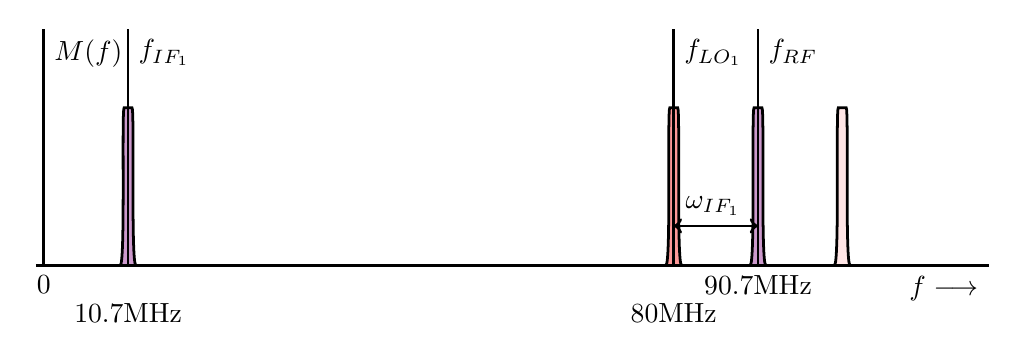
\begin{tikzpicture}[
        line width=1pt,
        sb/.style={text width=1.5cm, align=center,inner sep=0pt}]
        
    \DSBA{9.07}{0.1}{violet}{40}{2}
    \DSBA{8}{0.1}{red}{40}{2}
    \DSBA{10.14}{0.1}{red}{10}{2}
    \DSBA{1.07}{0.1}{violet}{40}{2}
    \draw   (-0.1,0) -- (12,0) node [below left] {$f \longrightarrow$}
            (0,0) node[below] {0} --++ (0,3) node [below right] {$M(f)$}
            (9.07,0) node[below] {90.7MHz} --++ (0,3) node [below right] {$f_{RF}$}
            (8,0) node[below,yshift=-10] {80MHz} --++ (0,3) node [below right] {$f_{LO_1}$}
            (1.07,0) node[below,yshift=-10] {10.7MHz} --++ (0,3) node [below right] {$f_{IF_1}$};
    \draw[<->] (8,0.5)--(9.07,0.5);
    \node[align=center, above] at (8.5,0.5) {$\omega_{IF_1}$};
                
    \end{tikzpicture}
\end{document}